\question[10] Andrea es ingeniera y quiere calcular la longitud de un lago con base en un diagrama (figura \ref{fig:lagoP}) que le han
enviado a su teléfono celular.¿Cuál es la longitud del lago?. Describe cada una de las
operaciones y razonamientos que te lleven a obtener esta medida.

\begin{minipage}{\textwidth}
    \begin{minipage}{0.45\textwidth}
        \begin{solutionbox}{6cm}
            Ya que comparten el ángulo opuesto por el vértice y los lados correspondientes son proporcionales, pues $\frac{160}{40} = \frac{120}{30}$.\\
            Entonces, la razon de semejanza entre los tri\'angulos es $r=\frac{160}{40}=4$, y la longitud del Lago ser\'a: \\ 55 m $\times r=220$ m.
        \end{solutionbox}
    \end{minipage}\hfill
    \begin{minipage}{0.45\textwidth}
        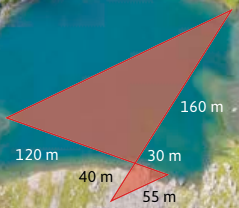
\includegraphics[width=0.9\linewidth]{Images/lagoP}
        \captionof{figure}{Vista fotográfica superior de la superficie del lago.}
        \label{fig:lagoP}
    \end{minipage}
\end{minipage}